\documentclass{ltjsarticle}

%%%%%%%%%%packages%%%%%%%%%%
%% colors and links
\usepackage[svgnames]{xcolor}
\usepackage[colorlinks,citecolor=DarkGreen,linkcolor=Blue,linktocpage,unicode]{hyperref} 

%% equations
%%%% math
\usepackage{amsmath,amsfonts,amssymb,amsthm}
\usepackage{mathtools}
\usepackage{mathrsfs}
\usepackage{bm}
\usepackage{cancel}
\usepackage{dsfont}
%%%% physics
\usepackage{siunitx}
\usepackage{physics}
%% positioning
\usepackage{array}
\usepackage{float}

%% table
\usepackage{booktabs}
\usepackage{multirow}
\usepackage{hhline}
\usepackage{caption}
\captionsetup{format=hang}
\usepackage{subcaption}

%% figure
\usepackage{graphicx}
\usepackage{tikz}
\usepackage{circuitikz}

%% decorations
\usepackage{titlesec}
\usepackage{picture}

%% framing
\usepackage{fancybox}
\usepackage{boites}
\usepackage{tcolorbox}
\tcbuselibrary{skins,theorems,breakable}

%% citation
\usepackage{cite}

%%%%%%%%%%optional settings%%%%%%%%%%

%%%%%図表並列%%%%%
\makeatletter
\newcommand{\figcaption}[1]{\def\@captype{figure}\caption{#1}}
\newcommand{\tblcaption}[1]{\def\@captype{table}\caption{#1}}
\makeatother

%%%%%itemization%%%%%
\renewcommand{\labelenumi}{\theenumi}
\renewcommand{\theenumi}{(\arabic{enumi})} % 箇条書きをローマ数字に

%%%%%%theorem environments%%%%%
\newtheoremstyle{mystyle}%   % スタイル名
    {}%                      % 上部スペース
    {}%                      % 下部スペース
    {\normalfont}%          % 本文フォント
    {}%                      % インデント量
    {\bf}%                  % 見出しフォント
    {.}%                      % 見出し後の句読点
    {\newline}%                     % 見出し後のスペース
    {\underline{\thmname{#1}\thmnumber{#2}\thmnote{(#3)}}}%
    % 見出しの書式 (can be left empty, meaning `normal')
\theoremstyle{mystyle} % スタイルの適用

\newtheorem{theorem}{定理}[section]
\newtheorem{definition}{定義}[section]
\newtheorem{proposition}[definition]{命題}
\newtheorem{corollary}[theorem]{系}
\renewcommand{\proofname}{証明}

\newtheorem{remark}{Remark. }[section]
\newtheorem{axiom}{公理}[section]
\newtheorem{conjecture}{Conjecture. }[section]

%%%%%%mathtools%%%%%
\mathtoolsset{showonlyrefs=true} % 被参照数式のみ数式番号割り振り
\numberwithin{equation}{section}

\makeatletter
\@addtoreset{equation}{section}
\makeatother

%%%%%%framing%%%%%

\newcommand{\lto}{\longrightarrow}
\newcommand{\lmto}{\longmapsto}
\newcommand{\btl}{\blacktriangleleft}
\newcommand{\btr}{\blacktriangleright}

\newcommand{\then}{\Rightarrow}
\newcommand{\incl}{\hookrightarrow}

%文字
\newcommand{\tbf}[1]{\textbf{#1}}

%括弧類
\newcommand{\lr}[1]{\langle{#1}\rangle}
\newcommand{\ler}[1]{\left({#1}\right)}
\newcommand{\blr}[1]{\left\{{#1}\right\}}
\newcommand{\slr}[1]{\left[{#1}\right]}

%積分測度
\newcommand{\pint}[1]{\int \mathcal{D}{#1}}
\newcommand{\moint}[1]{\int \frac{d^4{#1}}{(2\pi)^4}}
\newcommand{\xint}{\int d^4x}

%空間
\newcommand{\re}{\mathbb{R}}
\newcommand{\cpl}{\mathbb{C}}
\newcommand{\zet}{\mathbb{Z}}
\newcommand{\rpr}[1]{\mathbb{R}P^{#1}}
\newcommand{\cpr}[1]{\mathbb{C}P^{#1}}

%物理でよく使う記号
\newcommand{\kt}[1]{|{#1}\rangle}
\newcommand{\br}[1]{\langle{#1}|}
\newcommand{\brkt}[2]{\langle{#1}|{#2}|{#1}\rangle}
%%d次元作用
\newcommand{\sayou}[1]{\int d^{#1}x ~\mathcal{L}}

%矢印
\newcommand{\lto}{\longrightarrow}
\newcommand{\lmto}{\longmapsto}
\newcommand{\btl}{\blacktriangleleft}
\newcommand{\btr}{\blacktriangleright}

\newcommand{\thenarr}{\Rightarrow} %「ならば」の矢印
\newcommand{\incl}{\hookrightarrow} %inclusionの矢印
\newcommand{\ninf}{\xrightarrow{n\to\infty}} %n\to \inftyの矢印

%数学
%%何らかの空間の圏
\newcommand{\cat}[1]{\boldmath{{#1}}}

%slash_on_letter
\newcommand{\son}[1]{{\ooalign{\hfil$#1$\hfil\crcr\raise.167ex\hbox{/}}}}
%メモ: tikzsetでtikzコマンドを定義できる


%線分の中間に矢印を描くためのコマンド
%使い方: \draw[black, ->-={.5}{red}] (0,0)--(1,1);
%↑の時, (0,0)--(1,1)に伸びる線分の中間に赤い矢印が描かれる
\tikzset{->-/.style 2 args={
    postaction={decorate},
    decoration={markings, mark=at position #1 with {\arrow[thick, #2]{>}}}
    },
    ->-/.default={0.5}{}
}

\tikzset{-<-/.style 2 args={
    postaction={decorate},
    decoration={markings, mark=at position #1 with {\arrow[thick, #2]{<}}}
    },
    -<-/.default={0.5}{}
}


%3次元で交差する線分を描くコマンド
%上に来る線分を後に書く
%使い方: 
%\draw (0,0)--(1,1);
%\draw[overarc] (0,1)--(1,0);
\tikzset{
    overarc/.style={
        white, double=red, double distance=1.2pt, line width=2.4pt
    }
}


%

\title{Generalized symmetry Day3}
\author{Shuma NAKASHIBA}
\date{\today}

\begin{document}
\maketitle

\setcounter{tocdepth}{2}
\tableofcontents
\newpage
\section{(Temporal) Plan of this informal seminar}
In this week, I will try to show you the topics below: 
\begin{itemize}
    \item The remaining part of $d=3+1$ $U(1)$ Maxwell theory: 
    \begin{itemize}
        \item Gauging 1-form symmetry and $1$-form anomaly
        \item Duality between electric and magnetic $1$-form symmetry
        \item (If time allowed) the screening of string charge under the existence of matter field
    \end{itemize}
    \item The introduction to discrete higher-form symmetry: 
    \begin{itemize}
        \item General property of discrete gauge theory, in brief
        \item 3D toric code, as the manifestation of $\zet^e_2\times \zet^m_2$ $1$-form symmetry
    \end{itemize}
\end{itemize}
Also, there are other topics I want to cover (or, be covered by someone else): 
\begin{itemize}
    \item Spontaneous symmetry breaking of higher-form symmetry
    (There is a nice lecture note by McGreevy \cite{MG})
    \begin{itemize}
        \item General property (such as topological order, Goldstone boson), from the perspective of higher-form symmetry
        \item Examples (e.g. $Z_{N}$ gauge theory, or BF theory)
    \end{itemize}
    \item More about gauging higher-form symmetry and higher-form anomaly
    \item The classification of SPT phases with higher-form symmetry
    \item Lattice realizaton of higher-form symmetry
    \item More about higher group theory
\end{itemize}
I just intended to list up those topics as a suggestion for future seminar contents. 
Especially, the lattice one is totally unfamiliar to me and I want other people to cover that (, if necessary). \\\\
 We can also go into non-invertible way of generalization, like
\begin{itemize}
    \item Algebraic property of non-invertible symmetry: fusion category (or modular tensor category)
    \item Examples from rational CFT: 
    \begin{itemize}
        \item Ising CFT $\Leftrightarrow$ $\mathrm{TY}_{+}(\zet_2)$, its gauging and relationship to Majorana CFT 
        (see Shu-Heng's lecture note \cite{SHS})
        \item $c=1$ free compact boson, including Wess-Zumino-Witten model ($R=\sqrt{2}$) and orbifold CFT ($R=1/\sqrt{2}$)
    \end{itemize}
    \item Relationship to anyon braiding
    \item Lattice construction of non-invertible symmetry, its gauging, and relationship to LSM-type anomaly
    (e.g. Seifnashri's this work \cite{SS})
    \item Are there any others? (I don't know)
\end{itemize}
I think it's still enough if we cannot cover non-invertible side as long as we focus on higher-form side, 
but my interest may be a little bit more close to non-invertible stuff. \\\\
 As applications of those two generalizations, we may go further into
\begin{itemize}
    \item Higher gauging, and half-space gauging (though these two concept are essentially different)
    \item Symmetry TFT construction 
    \item Subsystem symmetry: "foliated" gauge field
    \item Lattice realization of various generalized symmetry (any kind of topics is appreciated)
\end{itemize}
although it will be very hard to cover the whole things (depending on the choice of next speakers).
%%%%%%%
%%%%%
%%%
%%
%
\newpage
\section{Short comment on last week's discussion}
\subsection{About the derivation of operator action on charged objects}
Last week, I tried to introduce a pure $3+1$-d $U(1)$ Maxwell theory and "derived" the action of an electric $1$-form operator on Wilson line 
from the definition of correlation function. 
I wrote the modified equation of motion as the form 
$d\star F = qg^2 \delta^3(\gamma)$. 
However, since both sides are not just numbers but operators acting on charged object
(note that our $2$-form electric symmetry ), 
we should actually write it instead as 
$$d\star F W(q, \gamma)= qg^2 \delta^3(\gamma) W(q, \gamma)$$
which makes much sense. 
This corresponds to considering Ward-Takahashi identity instead of just the classical equation of motion. 
\newpage
\section{Example: continued}
What is written below is totally the same as the one of last week's material 
(except the last subsubsection), 
so you may skip all of this. 
\subsection{$D=3+1$ $U(1)$ Maxwell gauge theory}
\subsubsection{Electric and Magnetic $1$-form symmetry}
As an example of higher-form symmetry appraring in physics, let's consider $U(1)$ pure Maxwell theory in $(3+1)$d spacetime. 
The action is given as 
\begin{align}
    S = -\frac{1}{2g^2} \int F\wedge \star F = -\frac{1}{4g^2}\int F_{\mu\nu}F^{\mu\nu}, 
    \label{U1pure}
\end{align}
where $F=dA$ is the 2-form field strength of gauge field $A$
\footnote{
    The representation of $F$ in a certain local trivialization is $F=\frac{1}{2}F_{\mu\nu}dx^\mu \wedge dx^\nu$. 
    Recall that, for any $k$-forms $\alpha, \beta$ defined on $n$-dimensional manifold (mfd, in short), 
    Hodge star operator is defined so that it satisfies
    $$\alpha\wedge (\star \beta)=\lr{\alpha, \beta}\mathrm{vol}, $$
    where $\langle ~ , ~ \rangle$ is the Gram determinant and $\mathrm{vol}$ is the $n$-dim volume form. 
    Using this, we obtain
    \begin{align}
        F\wedge \star F &= \lr{F, F} d^4 x~~(\mathrm{Note~that~we~consider~Wick-rotated~spacetime})\\
        &=frac{1}{4}\lr{F_{\mu\nu}dx^\mu\wedge dx^\nu, F_{\rho\sigma}dx^\rho\wedge dx^\sigma}d^4 x\\
        &=\frac{1}{4}F_{\mu\nu}F_{\rho\sigma}\det
        \begin{vmatrix}
            \lr{dx^\mu, dx^\rho} & \lr{dx^\nu, dx^\rho}\\
            \lr{dx^\mu, dx^\sigma} & \lr{dx^\nu, dx^\sigma}\\
        \end{vmatrix}\\
        &= \frac{1}{4}F_{\mu\nu}F_{\rho\sigma}(g^{\mu\rho}g^{\nu\sigma}-g^{\nu\rho}g^{\mu\sigma})\\
        &= \frac{1}{2}F_{\mu\nu}F^{\mu\nu} \ler{=\frac{1}{4}(F_{\mu\nu}F^{\mu\nu}-F_{\mu\nu}F^{\nu\mu})}. 
    \end{align}
}. Obviously, this action is invariant under gauge transformation $A\to A+d\lambda$ (since $F=dA$ transforms as 
$F\to F' = d(A+d\lambda) = dA + d(d\lambda) = dA +0$). 
The variation of $S$ under infinitesimal transformation $A\to A + \delta A$ is 
\begin{align}
    \delta S= -\frac{1}{2g^2}\int (d(\delta A)\wedge \star F + F\wedge \star d(\delta A) )
    =-\frac{1}{g^2} \int d(\delta A)\wedge \star F 
    =-\frac{1}{g^2}\int (\delta A \wedge d \star F + d(\delta A \wedge \star F)), 
\end{align}
where we used $\omega\wedge \star \eta = \eta\wedge \star \omega$ and 
$d(\omega\wedge \eta) = (d\omega)\wedge \eta + (-1)^{k_\omega} \wedge \eta$ for 
any $k_\omega$-form $\omega$ and $k_\eta$-form $\eta$. 
Therefore, the equation of motion for $A$ is $d\star F=0$. 
This means that we have a conserved $2$-form current $F$, implying that this pure $U(1)$ gauge theory has a $U(1)$ 1-form symmetry (a.k.a \textit{electric $1$-form symmetry}). \\
 Once we find a conserved current, we can write down the corresponding symmetry operator (which is topological) as an integral over closed $2$-dim surface 
($\lambda$ is a parameter specifying a certain $U(1)$ element)
\begin{align}
    U^{e}_{\lambda}(\Sigma_2) = \exp\blr{i\lambda\oint_{\Sigma}\frac{\star F}{g}}=: \exp\blr{i\lambda\oint_{\Sigma}J^e_2} ~~
    (\mathrm{just~a~choice~of~normalization}). 
    \label{electric1form}
\end{align}
The integral $\lambda\oint_{\Sigma}J^e_2$ is the "charge" of objects inside $\Sigma$. 
The charge quantization $\int_{\Sigma} \star F = 2\pi \zet$
\footnote{This quantization is nothing but the consequence of Chern-Gauss-Bonnet theorem in $n=2$ Riemannian mfd: \\
The integral of the Pfaffian of curvature $2$-form $\Omega$ over closed $2n$-dim mfd $\Sigma$ is given by the Euler number $\chi(\Sigma)$ as 
\begin{align}
    \int_{\Sigma} \mathrm{Pf}(\Omega) = (2\pi)^n \chi(\Sigma)~. 
\end{align}}
 tells us that the obtained symmetry is $U(1)$. \\
 The corresponding charged operator $W(q, \gamma)$ is extended along $1$-dim loop in spacetime, called \textbf{Wislon line}: 
  \begin{align}
    W(q, \gamma)=e^{iq\int_{\gamma}A}~(q\in \zet). 
  \end{align}
  The action of $U^{e}_\lambda(\Sigma)$ on this $W(q, \gamma)$ can be written as
  \begin{align}
    \lr{U^e_{\lambda}(\Sigma)W(q, \gamma)}=e^{iq\lambda\mathrm{Link}(\Sigma, \gamma)}\lr{W(q, \gamma)U^e_{\lambda}(\Sigma')}, 
    \label{ActionWlison} 
  \end{align}
  where $\mathrm{Link}(\Sigma, \gamma)$ is the \textit{linking number} of $\Sigma$ and $\gamma$
  \footnote{Formally, this is defined as follows. 
  First, we need to define "transverse intersection" of two submfds $U_q$ ($q$-dim) and $V_r$ ($r$-dim) on $d$-dim mfd $M$. 
  At every intersection point $p\in U_{q}\cap V_r$, if 
  their tangent spaces $T_p U_q$ and $T_p V_r$ together generate a $(q+r)$-dim subspace of $T_pM$, i.e., 
  $T_p U_q \otimes T_p V_r \subseteq T_p M$ for $\forall p\in U_{q}\cap V_r$, then 
  $U_q$ and $V_r$ are said to "intersect transversally". \\
 The linking number is defined by two oriented submanifolds $(U_q, V_r)$ in $d+1$-dim spacetime, 
   satisfying $q+r=d$. We further assume that, $U_q$ and $V_r$ themself do not have the intersecting point, 
   and each submanifold can be thought to form the boundary of a one-dim higher open manifold. 
   Then, by denoting $\partial W_{r+1}=V_r$, $U_q$ and $W_{r+1}$ can intersect in a finite number of points ${p_i}$ 
   (the set $\{p_i\}$ must be finite as long as we consider compact spacetime $M$). 
   Since $q+r+1=d+1$, the two tangent spaces $T_{p_i}U_q$ and $T_{p_i}W_{r+1}$ at each $p_i$ spans $T_{p_i}M$. 
   Thus, the orientations on $U_q$ and $W_{r+1}$ are used to define a new orientation to the neighborfood of $p\in M$. 
   If such an induced orientation is consistent with the original orientation of $M$, 
   then we define $\mathrm{sign}(p_i)=+1$, and if not, $\mathrm{sign}(p_i)=-1$. 
   The \textit{linking number} is defined by summing up the signs over all the intersecting point of $U_q$ and $W_{r+1}$: 
   \begin{align}
    \mathrm{Link}(U_q, V_{r}) = \delta_{r, d-q}\sum_{i}\mathrm{sign}(p_i). 
   \end{align}
   }
  . 
  \begin{figure}[!ht]
    \centering
    \resizebox{1\textwidth}{!}{%
    \begin{circuitikz}
    \tikzstyle{every node}=[font=\LARGE]
    \draw [ fill={rgb,255:red,168; green,198; blue,254} , line width=0.9pt ] (38,26.25) ellipse (7.75cm and 2.5cm);
    \draw [line width=0.9pt, short] (34.25,26.5) .. controls (33.5,33.75) and (28.75,30.75) .. (28.75,26.25);
    \draw [line width=0.9pt, short] (34,24) .. controls (33.25,20) and (29.25,20.5) .. (28.75,26.25);
    \draw [dashed] (34.25,26.25) .. controls (34.25,25) and (34.25,25) .. (34,24);
    \draw [->, >=Stealth] (28.75,26.75) -- (28.75,26.25);
    \draw [->, >=Stealth] (31.75,31) -- (31.5,31);
    \draw [->, >=Stealth] (31.5,21.5) -- (31.75,21.5);
    \node [font=\LARGE, color={rgb,255:red,227; green,36; blue,0}] at (34.25,26.5) {$\bullet$};
    \node [font=\LARGE] at (33.5,31) {$U_1$};
    \node [font=\LARGE] at (43,29.25) {$V_1 = \partial W_2$};
    \node [font=\LARGE] at (41,26) {$W_2$};
    \node [font=\LARGE] at (39.75,22) {$\mathrm{Link}(U_1, V_1)=1$};
    \draw [ fill={rgb,255:red,168; green,198; blue,254} , line width=0.9pt ] (61.25,26.5) ellipse (7.75cm and 2.5cm);
    \draw [line width=0.9pt, short] (57.25,26.75) .. controls (56.5,34) and (51.75,31) .. (51.75,26.5);
    \draw [line width=0.9pt, short] (57.5,24.25) .. controls (56.5,20.25) and (52.5,20.75) .. (51.75,26.5);
    \draw [dashed] (57.75,26.5) .. controls (57.75,25.25) and (57.75,25.25) .. (57.5,24.25);
    \draw [->, >=Stealth] (51.75,27) -- (51.75,26.5);
    \draw [->, >=Stealth] (54.75,31.25) -- (54.5,31.25);
    \draw [->, >=Stealth] (54.5,21.75) -- (54.75,21.75);
    \node [font=\LARGE, color={rgb,255:red,227; green,36; blue,0}] at (57.25,26.75) {$\bullet$};
    \node [font=\LARGE] at (56.5,31.25) {$\bar{U}_1$};
    \node [font=\LARGE] at (66,29.5) {$V_1 = \partial W_2$};
    \node [font=\LARGE] at (64,26.25) {$W_2$};
    \node [font=\LARGE] at (62.75,22.25) {$\mathrm{Link}(\bar{U}_1, V_1)=4$};
    \draw [line width=0.9pt, short] (57.75,26.5) .. controls (57,33.75) and (52.25,31.25) .. (52.25,26);
    \draw [line width=0.9pt, short] (58,24.25) .. controls (57,20) and (52.5,20.75) .. (52.25,26);
    \node [font=\LARGE] at (58.25,24.75) {};
    \node [font=\LARGE] at (58.25,24.75) {};
    \node [font=\LARGE] at (58.25,24.75) {};
    \draw [dashed] (58,24.25) .. controls (58.25,25) and (58.25,25.5) .. (58.25,26.5);
    \draw [line width=0.9pt, short] (58.25,26.5) .. controls (57.5,33.75) and (52.5,30.75) .. (52.75,26);
    \draw [line width=0.9pt, short] (58.5,24.25) .. controls (57.5,20) and (53,20.5) .. (52.75,26);
    \node [font=\LARGE] at (58.75,24.75) {};
    \node [font=\LARGE] at (58.75,25) {};
    \draw [dashed] (58.5,24.25) .. controls (58.75,25.25) and (58.75,25) .. (58.75,26);
    \draw [line width=0.9pt, short] (58.75,26.25) .. controls (57.75,33.5) and (53,30.25) .. (53.25,26.25);
    \draw [line width=0.9pt, short] (57,24.5) .. controls (57,22.5) and (54,20.75) .. (53.25,26.25);
    \draw [dashed] (57,24.5) .. controls (57.25,25.25) and (57.25,25.25) .. (57.25,26.75);
    \draw [->, >=Stealth] (52.25,26.75) -- (52.25,26.5);
    \draw [->, >=Stealth] (52.75,26.75) -- (52.75,26.5);
    \draw [->, >=Stealth] (53.25,26.75) -- (53.25,26.5);
    \draw [->, >=Stealth] (55.25,22.75) -- (55.5,22.75);
    \node [font=\LARGE, color={rgb,255:red,255; green,38; blue,0}] at (57.75,26.5) {$\bullet$};
    \node [font=\LARGE, color={rgb,255:red,255; green,38; blue,0}] at (58.25,26.5) {$\bullet$};
    \node [font=\LARGE, color={rgb,255:red,255; green,38; blue,0}] at (58.75,26.25) {$\bullet$};
    \end{circuitikz}
    }
    \caption{The illustration of the linking number in $3$d. }
    \label{fig:my_label}
    \end{figure}
  This action can be derived by considering the insertion of a Wilson line in spacetime. 
  Inserting a Wilson line (a source of electric flux) modifies the path integral as
  \begin{align}
    \int \mathcal{D}A~ e^{-S} \to \int \mathcal{D}A~ e^{iq\int_\gamma A} e^{-\frac{1}{2g^2}\int_{M_{4} F\wedge \star F}}
    =\int \mathcal{D}A~ e^{iq\int_\gamma \delta^3(\gamma)\wedge A -\frac{1}{2g^2}\int_{M^{4}} F\wedge \star F}, 
  \end{align}
where $\delta^3(\gamma)$ is a "3-form delta function" defined as $\int_{M_{3}^T}\delta^3(\gamma)=1$ 
for a 3-dim mfd $M_3^T$ which "transversely intersects" $\gamma$ only once. 
Then, the equation of motion for $A$ with the presence of Wilson line is
\begin{align}
    d\star F = qg^2 \delta^3 (x\in \gamma). 
\end{align}
We now integrate both sides of the EoM over a $3$-dim mfd $\Sigma^3$ whose boundary is $\partial \Sigma_3 = \Sigma_2$: 
\begin{align}
    (LHS)= \int_{\Sigma_3} d\star F = \oint_{\Sigma_2} \star F ~~(\mathrm{Stokes'~theorem}), 
\end{align}
\begin{align}
    (RHS)= qg^2 \int_{\Sigma_3} \delta(\gamma) = qg^2 \mathrm{Link(\Sigma_2. \gamma)}. 
\end{align}
Thus, by considering the "topological deformation" of $\Sigma_2$: 
\begin{figure}[H]
    \centering
    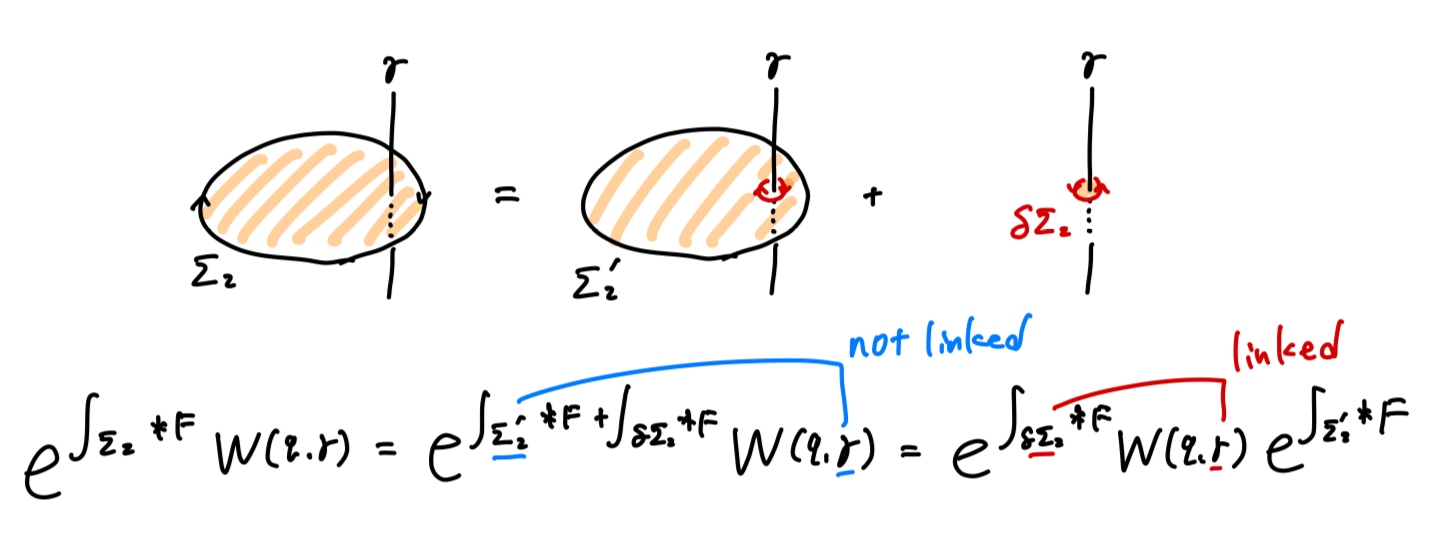
\includegraphics[width=0.8\textwidth]{ActionToWilsonLine.jpg}
    \caption{$\Sigma_2=\Sigma'_2\cup \delta \Sigma_2$, where $\Sigma_2$ is a boundary of infinitesimal $3$-dim mfd which links to $\gamma$. }
    \label{ActionToWlison}
\end{figure}
\noindent
Note that this deformation should be interpreted in path-integral formulation
\footnote{This means that we consider Ward-Takahashi identity as the current conservation, rather than Noether's theorem. 
In other words, we consider QFT rather than classical field theory. }
. Thus, we have 
\begin{align}
    \lr{\exp\blr{i\frac{\lambda}{g^2}\oint_{\Sigma_2}\star F}W(q, \gamma)}
    =\lr{e^{iq\lambda\mathrm{Link}(\Sigma_2, \gamma)}
    W(q, \gamma)\exp\blr{i\frac{\lambda}{g^2}\oint_{\Sigma'_2}\star F}W(q, \gamma)}, 
\label{WlisonLineCharge}
\end{align}
which is the same as \eqref{ActionWilson}. \\
 By the way, the action of $U^e_\lambda$ on $W(q, \gamma)$ can be seen as the shift of 1-form gauge field $A$ by 
 $A\mapsto A + a$, where $\oint_{\gamma} a =\lambda \mathrm{Link}(\Sigma_2, \gamma)$. 
 In fact, the associate current $\star J^e$ is the conjugate momentum of $A$, generating the shift of $A$. \\
 \\
  We can also consider the "dual" $1$-form symmetry: due to the Bianchi identity, we have $dF=0$ (that is, the pure Maxwell field is flat). 
 By regarding this identity as the conservation of $2$-form current $J^{m}_2 :=\frac{1}{2\pi}\star F$, we can write down the correponding symmetry operator as
 \begin{align}
    U^{m}_\lambda(\Sigma_2) = \exp\blr{i\lambda\oint_{\Sigma_2}\star J^m_2}
    =\exp\blr{i\lambda\oint_{\Sigma_2}\frac{F}{2\pi}}. 
 \label{magnetic1form}
 \end{align}
 This $1$-form symmetry is called \textit{magnetic $1$-form symmetry}. Its charged operator is the so-called \textbf{'t Hooft line}
 \begin{align}
    T_1(m, \gamma) := e^{im\int_{\gamma}\tilde{A}}, 
 \label{tHooft}
 \end{align}
 where $\tilde{A}$ is the dual gauge field defined by $\star F=d\tilde{A}$. 
 The action of the $1$-form magnetic symmetry on a 't Hooft line is completely analogous to the case of electric $1$-form symmetry: 
 \begin{align}
    \lr{U^{m}_\lambda(\Sigma_2)T_1(m, \gamma)}
    =e^{im\lambda\mathrm{Link}(\Sigma_2, \gamma)}\lr{T_1(m, \gamma)U^{m}_\lambda (\Sigma'_2)}. 
 \label{ActionTotHooft}
 \end{align}
 \subsubsection{Gauging $1$-form $U(1)$ symmetry}
 It is insightful to consider coupling "background gauge field" to our conserved $2$-form currents, as we have done in the case of ordinary $U(1)$ gauge theory. 
 In this case, the dynamic field $A$ is $1$-form, the conserved current is $2$-form, and the background gauge field to be coupled is $2$-form. 
 This is done by adding to the action integral
\footnote{詮: 系の力学を記述する「作用積分」と, 演算子の場に対する「作用」を区別するために, 以降は(文脈から明らかな場合を除いて)前者を"action integral"と呼ぶことにします. }
 the term $\int B^e_2\wedge \star J^e_2$ and $\int B^m_2\wedge \star J^m_2$ respectively, 
where $B^e_2$ and $B^m_2$ are the $2$-form background gauge field of $1$-form electric/magnetic symmetry.  
The possible form of the modified action integral would be 
\begin{align}
    S_1=\frac{1}{2g^2}\int (F-B^e_2)\wedge \star (F-B^e_2) 
    +\frac{i}{2\pi}\int B^m_2 \wedge F
    =\frac{1}{2g^2}\int F\wedge \star F -\frac{1}{g^2} B^2 \wedge F
    +\frac{1}{2g^2}\int B^e_2\wedge B^e_2 + 
    \frac{i}{2\pi}\int B^m_2\wedge F. 
\label{Gauging1formSym}
\end{align}
The new term $\int B^e_2\wedge B^e_2$ is to ensure the invariance of the kinetic term $\int F\wedge \star F$
under the gauge transformation $A\to A+ \lambda^e_1,~ B^e_{2}\to B^e_2 + d\lambda^e_1$ ($\lambda^e_1$ : some (non-closed) $1$-form). 
Note that, this term does not affect the dynamics of the theory unless we treat $B^e_2$ and $B^m_2$ just as "background" fields 
(so, the choice of such an additional term is not unique: we will point out that again below). 
This action is invariant under magnetic $1$-form transformation $\tilde{A} \to \tilde{A}+\lambda^{m}_1, ~B^m_2\to B^m_2 + d\lambda^m_1$, 
but not invariant under electric $1$-form transformation $A\to A+ \lambda^e_1,~ B^e_{2}\to B^e_2 + d\lambda^e_1$: 
\begin{align}
    \delta S_1 = \frac{i}{2\pi}\int B^m_2\wedge d\lambda^e_1. 
    \label{eleAno}
\end{align}
Thus, the magnetic $1$-form symmetry can be "gauged" consistently under this $S_1$ while the electric $1$-form cannot. \\
 Another choice of modification might be
\begin{align}
    S_2 = -\frac{1}{2g^2}\int (F-B^e_2)\wedge \star (F-B^e_2)
    +\frac{i}{2\pi}\int B^m_2\wedge(F-B^e_2), 
\end{align}
The action is in turn invariant under electric $1$-form symmetry, 
but not under the magnetic $1$-form transforastion $
A^m\to A^m + \lambda^m_1, ~B^m_2\to B^m_2 + d\lambda^m_1$ : 
\begin{align}
    \delta S_2 = \frac{i}{2\pi}\int -d\lambda^m_1\wedge B^e_2. 
    \label{magAno}
\end{align}
Combining the two observation, we can see that 
we cannot make both electric and magnetic $U(1)$ $1$-form symmetry simultaneous by any choice of additionallocal term. 
Such a situation is described as that the action of $3+1$-d Maxwell theory has a mixed 't Hooft anomaly of $U(1)^{(1)}_e$, $U(1)^{(1)}_m$. \\\\
 Let us see the mixed anomaly \eqref{magAno} from the inflow pitcure briefly. 
We consider the following "anomaly inflow action" in five dimension: 
\begin{align}
    S_{\mathrm{inflow}} = -\frac{i}{2\pi}\int_{N_{5}} B^{m}_2\wedge dB^e_2, 
\end{align}
where $\partial N_5 = M_4$ is our spacetime manifold. By the background gauge transformation $B^m_2 \to B^m_2 + d \lambda^m_1$, we have
\begin{align}
    \delta S_{\mathrm{inflow}} &= -\frac{i}{2\pi}\int_{N_5} d\lambda^m_1 \wedge dB^e_2 \\
    &=-\frac{i}{2\pi}\int_{N_5}\blr{d(d\lambda^m_1\wedge B^e_2)-d^2\lambda^m_1 \wedge dB^e_2}\\
    &=-\frac{i}{2\pi}\int_{\partial N_5}d\lambda^m_1\wedge B^e_2 + 0~~
    (\because \mathrm{Stokes' thm})\\
    &=-\frac{i}{2\pi}\int_{M_4}d\lambda^m_1\wedge B^e_2, 
\end{align}
which is just the same as $\delta S_2$ in \eqref{magAno}. 
Therefore, we can add $-S_{\mathrm{inflow}}$ in our action integral to cancel the mixed 't Hooft anomaly 
in the boundary $M_4$. \\\\
 More generally, when a $U(1)$ $p$-form gauge field $A_p$ and its $D-p$-form dual with action integral
$$S=\int_M \frac{1}{2g^2}F_{p+1}\wedge \star F_{p+1}, ~~F_{p+1} = dA_p$$
are simultaneously coupled to a background gauge field $B_{p+1}^{(e)}$ and $B_{D-p-1}^{(m)}$, 
then the action integral
\begin{align}
    S=\int \frac{1}{g^2}(F_{p+1}-B^{(e)}_{p+1})\wedge \star(F_{p+1}-B^{(e)}_{p+1})+\frac{i}{2\pi}F_{p+1}\wedge B^{(m)}_{D-p-1}
\end{align}
is not invariant under background gauge transformation $B^{(e)}_{p+1}\to B^{(e)}_{p+1} + \delta B^{(e)}_{p+1}$: 
\begin{align}
    \delta S = i\int \Lambda^{(e)}_{p+1} \wedge \frac{B^{(m)_{D-p-1}}}{2\pi}, 
\end{align}
and is not canceled by any counter term. 
However, we can add the term of the integral of $D+1$-form
\begin{align}
    S_{\mathrm{inflow}} = \frac{i}{2\pi}\int_{N} B^{(e)}_{p+1}\wedge dB^{(m)}_{D-p-1} ~~(\partial N = M)
\end{align}
to cancel the above $\delta S$. \\
%%%%
%%%%
\subsubsection{Electric-magnetic duality}
This part is mainly based on \cite{TD}. Please see his video for detail. \\
 Let's now consider the following action integral, whose dynamical gauge field is $\tilde{A}$:
\begin{align}
    S[\tilde{A}, F]
    =-\frac{1}{2g^2}\int F\wedge \star F + \frac{i}{2\pi}\int d\tilde{A}\wedge F. 
\label{dualityAction}
\end{align}
The action is the form of coupling magnetic $2$-form current $\star J^{m}_2 = \frac{1}{2\pi}F$ to dynamical gauge field $\tilde{A}$. 
"Integraling out" the $\tilde{A}$ field obviously reproduces the action \eqref{U1pure}, 
which means that gauging magnetic $1$-form symmetry $U^{(1)}_m$ yields an electric $1$-form symmetry $U^{(1)}_e$. 
Mathematically, gauging the symmetry $\mathcal{G}$ in a theory $\mathcal{T}$ gives 
another theory $\mathcal{T}/\mathcal{G}$, whose symmetry is given as the Pontryagin dual: 
\begin{align}
    \hat{\mathcal{G}}:= \mathrm{Hom}(\mathcal{G}, U(1)). 
\end{align}
$\mathrm{Hom}$ is the set of (group) homomorphisms (群準同型) between two groups. 
For abelian group, the Pontryagin dual is known to be the same as the original one: 
$\hat{A}\simeq A$ ($A$: abelian). 
Therefore, by gauging (magnetic) $1$-form $U(1)$ symmetry, 
we succeeded in obtaining another (electric) $1$-form $U(1)$ symmetry as its dual. 
\\
 Another way to study the relation of $U^{(1)}_e$ and $U^{(1)}_m$ is to consider the equation of motion for $\tilde{A}$ in the action \eqref{dualityAction}, 
which is
\begin{align}
    \frac{i}{g^2}\star F = -\frac{1}{2\pi}d\tilde{A} \ler{=: \frac{1}{2\pi}\tilde{F}}. 
\end{align}
By using the property of Hodge star operator for arbitrary $p$-form $\omega$, 
$\star\star \omega = (-1)^{p(d+1-p)}\omega$ (for our case $p=2$), we can also have
\begin{align}
    \star \tilde{F}= -\frac{2\pi i}{g^2}F. 
\end{align}
Then we can rewrite the action \eqref{dualityAction} using $\tilde{A}$ only: 
\begin{align}
    \tilde{S}[\tilde{A}]
    &=-\frac{1}{2g^2}\int \ler{\frac{g^2}{2\pi i}\star \tilde{F}}\wedge \ler{\frac{g^2}{2\pi i}\tilde{F}} + \frac{i}{2\pi}\int \tilde{F}\wedge \ler{\frac{g^2}{2\pi i}\star \tilde{F}}\\
    &=-\frac{g^2}{8\pi^2}\int \tilde{F}\wedge \star \tilde{F}. 
\end{align}
Then, this $\tilde{S}[\tilde{A}]$ becomes the same form of the original action under the EoM of dynamic field $\tilde{A}$. 
But the coupling constant is different: for the theory of $\tilde{S}$, 
\begin{align}
    \frac{1}{2\tilde{g}^2} = \frac{g^2}{8\pi^2} ~\to~\tilde{g}^2 = 4\pi^2 / g^2.  
\end{align}
This means that, when the original coupling constant of the original dynamical field $A$ becomes smaller, 
the "dual" coupling constant of the dual field $\tilde{A}$ becomes larger. \\\\
%\color{red}
%THE FOLLOWING IS INCOMPLETE AND MAY CONTAIN INCORRECT INFORMATION, SO IT MAY BE GOOD TO JUST SKIP THIS. \\
%\color{black}
% Some literature calls this duality of electric and magnetic $1$-form symmetry as 
%"S-duality". 
%Let me explain why it is called S-duality, with referring to the relationship to modular transformation. 
%Consider a $1+1$-d torus of genus $1$, which is depicted in $\mathbb{C}$ as
%\begin{tikzpicture}
%    \draw [line width=0.5pt] (0,0) rectangle (0.5,0.5);
%    \draw [line width=0.3pt, ->] (0,0) -- (0,0.25);
%    \draw [line width=0.3pt, ->] (0.5,0) -- (0.5,0.25);
 %   \draw [line width=0.3pt, ->] (0,0.5) -- (0.22,0.5);
  %  \draw [line width=0.3pt, ->] (0,0) -- (0.22,0);
  %  \draw [line width=0.3pt, ->] (0,0.5) -- (0.32,0.5);
  %  \draw [line width=0.3pt, ->] (0,0) -- (0.32,0);
%\end{tikzpicture}
% with each pair of horizontal edges identified. 
% Take $z=0, 1, \tau, 1+\tau$ as vertex coordinates, then this $\tau$ is the modulo of the torus. 
% The modular transformation is generated by following two transformations:
% \begin{align}
%    &T: \tau \mapsto \tau + 1, \\
%    &S: \tau \mapsto -\frac{1}{\tau}. \\
% \end{align}
%When we insert a defect loop in one direction as
%\begin{tikzpicture}
%    \draw [line width=0.5pt] (0,0) rectangle (0.5,0.5);
%    \draw [line width=0.3pt, ->] (0,0) -- (0,0.25);
%    \draw [line width=0.3pt, ->] (0.5,0) -- (0.5,0.25);
%    \draw [line width=0.3pt, ->] (0,0.5) -- (0.22,0.5);
%    \draw [line width=0.3pt, ->] (0,0) -- (0.22,0);
%    \draw [line width=0.3pt, ->] (0,0.5) -- (0.32,0.5);
%    \draw [line width=0.3pt, ->] (0,0) -- (0.32,0);
%    \draw [line width=0.5pt, ->, color=red] (0.25,0) -- (0.25,0.5);
%\end{tikzpicture}
%, then $T$ and $S$ are depicted as follows respectively: 
%figure
% Let's go back to our case, $d=3+1$ Maxwell theory. 
%There are two types of topological codim-2 operators: 
%Wilson loop and t' Hooft loop. 
%%%%ちょっとまって, 怪しくなってきた
%%%%d=3=2+1の話だったかもしれない
%When a Wilson loop is extended vertically to time direction, 
%and the time direction is compactified, 
%then the charged operator 
%%%%%%S-dualityの正確な意味するところを知っておくべき
 The duality picture gives us an important viewpoint of the symmetry: 
symmetry operators act on defect operators, which generates the symmetry of the system. 
In other words, the algebra of symmetry operators is the representation of the symmetry, 
whose representation space is spanned by defect operators. 
Generally, this algebraic structure is not necessarily group-like 
(called "higher group"), 
so we will go on a journey to the representation theory of category (圏) 
in order to study the physics under generalized symmetry. 
\section{Screening of $1$-form charge}
Theories with higher-form symmetry have some extended operators
\footnote{Note that, we frequently use the term "operators" and "defects" interchangeably. } in more than $1$ dimension. 
For such extended operators, we can consider the \textbf{screening} of a certain operator $\mathcal{O}_p$ to another one $\mathcal{O}_p$. 
This will actually turn out to be a strong method to perform higher-form symmetries of gauge theories. \\
 The screening is defined as follows: 
\begin{definition}{Screening}
    A $p$ ($\geq 1$)-dimensional operator $\mathcal{O}_p$ can be "\textbf{screened} 
    to another $p$-dimensional $\mathcal{O}'_p$ if we can insert a $(p-1)$-dimensional operator $\mathcal{O}_{p-1}$ 
    between $\mathcal{O}_p$ and $\mathcal{O}'_p$, depicted as follows: 
    \begin{figure}[H]
        \centering
        \begin{tikzpicture}
            \draw[line width=0.9pt] (-2,0)--(2,0); 
            \node[color=red] at (0,0) {$\bullet$};
            \node[color=black] at (-2,0) {$\bullet$};
            \node[color=black] at (2,0) {$\bullet$};
            \draw[line width=0.9pt] (-2,0)--(2,0); 
        \node[color=red] at (0,0) {$\bullet$};
        \node[left] at (-2,0) {$\mathcal{O}_p$};
        \node[right] at (2,0) {$\mathcal{O}'_p$};
        \node[above, color=red] at (0,0) {$\mathcal{O}_{p-1}$};
        \end{tikzpicture}
        \caption{Screening of $1$-form charged defect by $0$-form defect. }
    \end{figure}
    Moreover, a $p$-dim $\mathcal{O}_p$ is \textbf{completely screened} if 
    is can end on a $(p-1)$-dim operator.       
\end{definition}
Some literatures (such as \cite{SSN}) uses the term \textit{screened} to mean \textit{completely screened} 
defined above. \\
 The important point of this screening is that, 
if one operator $\mathcal{O}_p$ is screened to another $\mathcal{O}'_p$, then they have the same $p$-form charge. 
In particular, for a \textit{completely screended} operator $\mathcal{O}_p$,
 the $p$-form charge becomes zero, which is pictorically apparent: 
\begin{equation}
    \begin{split}
        &
 \begin{tikzpicture}
    \draw[line width=0.9pt] (-2,0)--(-1.4,0); 
            \draw[color=blue] (-1,0) circle (0.3 and 1); 
            \fill[white] (-0.8, -0.1) rectangle (-0.6, 0.1);
            \draw[line width=0.9pt] (-1.2,0)--(0,0);
            \node[color=red] at (0,0) {\bullet}; 
            \node at (-2,0) {\bullet}; 
            \node[left] at (-2,0) {$\mathcal{O}_p$}; 
            \node[color=red, right] at (0,0) {$\mathcal{O}_{p-1}$}; 
 \end{tikzpicture}
 \begin{tikzpicture}
    \node at (-3,0) {=};
        \draw[line width=0.9pt] (-2,0)--(0,0); 
            \draw[color=blue] (-1,0) circle (0.05 and 0.1); 
            \node[color=red] at (0,0) {\bullet};
            \node[left] at (-2,0) {$\mathcal{O}_p$}; 
            \node[color=red, right] at (0,0) {$\mathcal{O}_{p-1}$}; 
 \end{tikzpicture}
 \begin{tikzpicture}
    \node at (-3,0) {=};
    \draw[line width=0.9pt] (-2,0)--(0,0); 
        \node[color = blue] at (-1,0) {\bullet};
        \node[color=red] at (0,0) {\bullet};
        \node[left] at (-2,0) {$\mathcal{O}_p$}; 
        \node[above, color=blue] at (-1,0) {$R_g(\mathcal{O}_p)$}; 
        \node[color=red, right] at (0,0) {$\mathcal{O}_{p-1}$}; 
\end{tikzpicture}\\
&
\begin{tikzpicture}
    \node[rotate=90] at (-1.5,0) {=};
    \node[color=white] at (-3,0) {=};
    \node[color=white] at (0,0) {=};
\end{tikzpicture}\\
&
\begin{tikzpicture}
    \draw[line width=0.9pt] (-2,0)--(0,0);
    \draw[color=blue] (1.4,0) circle (0.3 and 1);
            \node[color=red] at (0,0) {\bullet}; 
            \node at (-2,0) {\bullet}; 
            \node[left] at (-2,0) {$\mathcal{O}_p$}; 
            \node[color=red, right] at (0,0) {$\mathcal{O}_{p-1}$}; 
 \end{tikzpicture}
 \begin{tikzpicture}
    \node at (-3,0) {=};
    \draw[line width=0.9pt] (-2,0)--(0,0);
    \node[color=blue] at (1.4,0) {\bullet};
            \node[color=red] at (0,0) {\bullet}; 
            \node at (-2,0) {\bullet}; 
            \node[left] at (-2,0) {$\mathcal{O}_p$}; 
            \node[color=red, right] at (0,0) {$\mathcal{O}_{p-1}$}; 
 \end{tikzpicture}
\end{split}
\end{equation}
In other words, when some defects are completely screened by $1$-dim lower ($1$-codim higher) objects, 
then the defects cease to be topological. 
This can be interpreted as the breaking of $p$-form symmetry induced by lower-dimensional objects of 
nontrivial vacuum expected value (vev). Here we stop by just mentioning the relationship between screening and SSB. 
\subsection{studying $p$-form symmetry from (absense of) screening}
We can say the converse of the above statement: 
if $\mathcal{O}_p$ and $\mathcal{O}'_p$ are not screened to each other, 
then we can construct a representation of $p$-form symmetry action on $p$-dim charged defects,  
so that $\mathcal{O}_p$ and $\mathcal{O}'_p$ have a different charge under it. \\\\
 In practice, we define the "symmetry" under the following strategy. 
We first identify two $p$-dim operators if they are related by screenings. 
Then, we can define the equivalence classes of $p$-dim operators by the above identification (we denote the set of all eq. classes as $D_{p}$). 
We can induce a ring (環) strucure on the set $D_p$, but for many cases the $D_p$ can be an abelian group. \\
 In our setup, we must have a $p$-form symmetry whose charge distinguishes 
objects of different equivalence classes i.e. different elements of $D_p$. 
Such a $p$-form symmetry is the group $G^{(p)}=\hat{D}_p$ (Pontryagin dual). 
In contrast, the possible charges under this $p$-form symmetry group forms the group $D_p$ itself. 
By definition, this corresponds to elements of the equivalence class of charged operators $\slr{\mathcal{O}_p}\in D_p$ 
(the equivalence class of charged operators are labeled by their charges). \\\\
 For the case of $1$-form symmetries, line operators may be screened by local (0-form) operators. 
The global form of the gauge group determines what representation of local operators are allowed, 
which in turn specifies what set of line operators are screened (endable at local operators). 
To be more concrete, consider the Wilson lines of a gauge theory 
which transform in a representation $R$ of the gauge group
\begin{align}
    W_R(q^a, \gamma) = \mathrm{Tr}_{R}~Pe^{iq^a\int_\gamma ~A^a}. 
\end{align}
In other words, they are world-lines along the path $\gamma$ of heavy probe particles with rep. $R$. 
If a Wilson line $W_R$ is endable on a local operator $\mathcal{O}_R$ which transforms in the same representation $R$, 
then the $\mathcal{O}_R$ corresponds to an annihilation operator of the heavy probe particle. 
If a theory does not have such a particular operator representation, 
the Wilson line does not end, and carries a non-trivial charge under the $1$-form symmetry. 
\subsection{Maxwell theory, with matter field}
This example is based on \cite{LBLBLFTLGDGAPHT}. 
Consider a $d+1$-dimensional gauge theory with $U(1)$ gauge group, along with a matter field $\phi$ with charge of a certain value $q\in \zet$ 
under the $U(1)$ gauge group. We will see that the introduction of this $\phi$ breaks the $U(1)$ 1-form symmetry to its $\zet_q$ subgroup 
(then, this theory turns out to have a $\zet_q$ 1-form symmetry). \\\\
 The key point is that, the matter field $\phi$ gives rise to a 
\textit{non-genuine} local operator $\phi(x)$ that screens a Wilson line of charge $q$ as shown: 
\begin{figure}[H]
    \centering
    \begin{tikzpicture}
        \draw[line width=0.9pt] (-2,0)--(2,0);
        \node[color=red] at (2,0) {$\bullet$};
        \node[color=red, right] at (2,0) {$\phi(x)$};
        \node[left] at (-2,0) {$W(q, \gamma)$};
    \end{tikzpicture}
    \label{fig:label}
\end{figure}
Here, a \textit{non-genuine} $q$-dimensional operator is defined to be an operator that is attached to a collection of $p$($>q$)-dimensional operators. 
An insertion of a genuine field $\phi(x)$ cannot be done because it is not gauge invariant. 
Still, we can consider the gauge-invariant way to insert $\phi$, by attaching it to a Wilson line 
on a (semi-)finite Line $L$ at $x=\partial L$. 
In fact, the gauge transformation $A(x)\mapsto A(x)-\frac{d\theta(x)}{2\pi}$ gives
\begin{align}
    \phi(x)&\mapsto e^{iq\theta(x)}\phi(x), \\
    W(q, \gamma)=\exp\ler{2\pi iq\int_L A}&\mapsto \exp\ler{- iq\int_L d\theta}W(q, \gamma)
    =\exp\ler{-iq\int_{\partial L} \theta}W(q, \gamma)
    =e^{-iq\theta(x)}W(q, \gamma), \\
\end{align}
thus the two factors cancel each other to make $\phi(x)W(q, \gamma)$ gauge invariant. \\
 Similarly, by inserting a power $\phi^n$, we can screen a Wilson line of charge $q_0 + nq$ to another line of charge $q_0$. 
 Therefore, when we have a matter field $\phi$ of charge $q$, the charge of $1$-form symmetry (charge carried by Wilson lines) is meaningful only modulo $q$, 
 and the group of equivalence classes of unscreened line operators becomes the quotient by $q\zet$: 
 $D_1 = \frac{\zet}{q\zet} = \zet_q$. 
 The group $\zet$ in numerator is the group of equivalence classes of Wilson lines before screening (note that the action of $1$-form symmetry on Wilson lines is defined by linking number), 
 and $\zet_q$ in the denominator is the group of completely screened Wilson lines by $\phi$ (with $0$-form charge $q$). 
 This is how a $0$-form charged operator can screen the charge of $1$-form operators. \\\\
  As is seen before, the $1$-form symmetry distinguishing the $\zet_q$-valued charge of (screened) Wlison lines 
 is the Pontryagin dual $G^{(1)} = \hat{\mathbb{Z}_q}\sim \zet_q$
 \footnote{The Pontryagin dual of $\zet_q$ is $\mathrm{Hom}(\zet_q, U(1))\simeq \zet_q$. 
 In fact, if we label the element of $\zet_q$ as $g_{n} = e^{\frac{2\pi i n}{q}}~(n=0, 1, \cdots, q-1)$, 
 then the possible homomorphism takes the form of
 \begin{align}
    \varphi_N: \zet_q \to U(1), ~~ \varphi_{N}(g_n) = (e^{\frac{2\pi i n}{q}})^{N}~~(N=0, 1, \cdots, q-1). 
 \end{align}
 Thus, the set of such $\varphi$s is equivalent to $\zet_q$. \\
 More generally, if $G$ is a finite abelian group, then we can have
\begin{align}
    \hat{G} = \mathrm{Hom}(G, U(1))\simeq G. 
\end{align}
Note that $G$ must be finite. In fact, we can see $\hat{\zet} = U(1)$ by considering the map
\begin{align}
    \varphi_\alpha: \zet \to U(1), ~~ n\mapsto e^{in\alpha}. 
\end{align}
The label $\alpha$ of $\mathrm{Hom}(\zet, U(1))$ takes value on $[0, 2\pi)$, then 
the set of $\varphi_\alpha$s form a $U(1)$ group.}. 
 The corresponding codim-2 topological operators generating this $1$-form symmetry are 
 a subset of the operators in the case of pure $U(1)$ gauge theory, given by
 \begin{align}
    U^e_{n}(\Sigma_{d-2}) = \exp\ler{
        \frac{i}{g^2}\frac{2\pi n}{q}\int_{\Sigma_{d-2}}\star F
    }, ~~ n\in \blr{0, 1, \cdots, q-1}. 
 \end{align}
These operators acts on Wilson lines of charge $q$ trivially, as the phase factor obtained by action becomes
\begin{align}
    \exp\ler{i\frac{2\pi n}{q}\cdot q \cdot \mathrm{Link}(\Sigma_{d-2}, \gamma)} = \exp(2\pi i n \cdot \mathrm{Link}(\Sigma_{d-2}, \gamma))=1, 
\end{align}
since the linking number is always an integer. 
\section{More About Higher-Form Symmetry}
\small
Maybe this will be skipped or given talks by another person. 
\subsection{Anomaly of Higher-Form Global Symmerty}
\subsubsection{Anomaly in general}
\subsection{Spontaneous Symmetry Breaking of Higher-form Symmetry}
\newpage
\section{Discrete Gloal Symmetry}
So far, we have only considered systems with continuous symmetry. 
In that case, we can find conserved $(d-p)$-form current, or closed $d$-form explicitly, 
by considering infinitesimal transformations of group elements parametrized by continuous numbers. \\
 However, we cannot do in the same manner for the case of discrete symmetry, 
such as $\zet_2$ or $\zet_N$. 
Indeed, the concept of "infinitesimal transformation" is totally nonsense for discrete symmetry 
since all the elements are "finitely separated"
\footnote{
    More precisely, 
    discrete group is equipped with discrete topology (離散位相) while 
    continuous group can have the structure of metric space (距離空間). 
    Especially, Lie group is equipped with differential structure (微分構造). 
} from identity. 
Then, how can we characterize the symmetry of discrete group? 
Remember that the theory with (generalized) symmetry has symmetry operators which are topological, 
and symmetry action on charged objects known as defect operators is defined. 
For continuous case, we can construct such topological operators explicitly from the conserved current. 
How can we find such topological operators in the case of discrete symmetry? \\
 Note that, even in the case of discrete symmetry, 
we can still have the notion of "defect operator". 
There are several characterization of defect operators. 
One way is the following. \\
 Another way is from the perspective of gauging: the insertion of symmetry defect operators corresponds to turning on a background gauge field. 

%長い
\subsection{BF theory}
%BF theoryの簡単な例を知りたい
Let's consider $\zet_{N}$ $p$-form gauge theory. 
One way to construct such a theory is called \textbf{BF theory}, 
which is a constrained $U(1)$ gauge theory 
so that only $\zet_N$ gauge fields contribute to the path integral 
(note that $\zet_N \subset U(1)$ as a subgroup). 
In this case, we only encounter Wilson lines whose test charges only have a meaning modulo ${N}$. \\
 We will consider a $D=d+1$-dimensional theory of a $U(1)$ $p$-form gauge field $A_p$ with a $U(1)$ $(d-p-1)$-form background gauge field. 
The action is of the form 
\begin{align}
    S=\frac{iN}{2\pi}\int B_{d-p}\wedge dA_p, 
\end{align}
which is invariant under the transformation 
$A_{p}\mapsto A_p + d\Lambda_{p-1}$ and $B_{d-p}\mapsto B_{d-p} + d \Lambda_{d-p-1}$. 
We normalize the $q$-form ($q=p$ or $d-p$) so that $\oint_{\Sigma_{q+1}}\frac{d\Lambda_q}{2\pi}\in \zet$. 
The equation of motion tells us that the gauge fields $A_p$, $B_{d-p}$ are flat: 
\begin{align}
    N\frac{dA_p}{2\pi} = 0, ~~ N\frac{dB_{d-p}}{2\pi} = 0. 
\end{align}
The equation of motion restrics the path integral to the sum only over $\zet_N$ gauge fields. 
\subsubsection{Discrete Global Symmetry of BF Theory}
The EoM of BF theory seems to be trivial, but we still have the field configurations 
where the holomomies are $\zet_N$-valued: 
\begin{align}
    N
\end{align}
\subsection{Example From Lattice: 3D Toric Code}
Now we will see the example of lattice models which have some higher-form symmetries. 
3D toric code
\footnote{As is mentioned last week, 
when the target space dimension is $D$, 
the possible (higher-form) symmetries are of $p=0, 1, \cdots, D-2$. 
Therefore, 2D toric code cannot have any higher-form symmetry, 
but $3D$ toric code can. }
, whose target space is 3-dimensioanl
\footnote{Note that toric code model is not necessary defined on a torus. 
In fact, the Hamiltonian can be defined on any square lattice, 
as long as it has vertices and plaquettes. }
, is known as the example of $1$-form 
discrete global symmetry: $\zet^{e}_2\times \zet^m_2$. 
\subsubsection{Brief review of toric code model}
The \textbf{toric code} model is constructed on 
an arbitrary dimensioanl lattice (typically square lattice), with periodic boundary condition on both directions 
(i.e. the Hilbert space is on torus $T^2$). 
We put a qubit on every link. 
The Hamiltonian is 
\begin{align}
    H=-\sum_j A_j - \sum_p B_p, 
    \label{TCmodel}
\end{align}
where $j$ and $p$ is the index of site and plaquette respectively, 
$A_{j}\equiv \prod_{l:\mathrm{link~ending~at~j}} Z_l$ is defined for every site $j$, 
and $B_{p}\equiv \prod_{l:\mathrm{bdy~of~p}} X_l$ is for every plaquette $p$. 
$A_j$ and $B_p$ are sometimes called "Gauss law operator" and "flux operator" respectively. \\
 All of those operators $A_j$ and $B_p$ commute with each other since 
they all share an even number (0, 2, or 4) of $X$s and $Z$s 
(so we always have $(-1)^{\mathrm{even}}$ factor). 
Then, we can diagonalize all terms in \label{TCmodel} simultaneously. \\
 Let's consider states whose eigenvalue of $A_j$ is 1 for every vertex $j$. 
For such states, all vertex should be associated with an even number of $X_l$s ending on it. 
The states satisfying this condition are "closed-string states", 
where all lines of electric flux are closed and have no charges to end on. 
Therefore, the groundstate of the toric code model is degenerated as many as the possible closed loop configuration, 
which is the order of the exponential of the system size. \\\\
 The excitation of toric code is created by open strings of $Z$s or $X$s. 
When we have a $Z$ on a link $(j_1, j_2)$, then 
the eigenvalues of $A_{j_1}$ and $A_{j_2}$ are flipped $1\to -1$, 
and the total energy is increased by $4$. 
In this case, we say that the $Z$ creates a pair of \textit{$e$-excitations} at vertex $j_1$ and $j_2$. 
Similarly, a $X$ on a link $(j_1, j_2)$ creates 
a pair of \textit{$m$-excitations} at plaquette $p_1$ and $p_2$, 
where $p_1$ and $p_2$ are the plaquettes sharing the link $(j_1, j_2)$. 
 \begin{figure}[H]
     \centering
     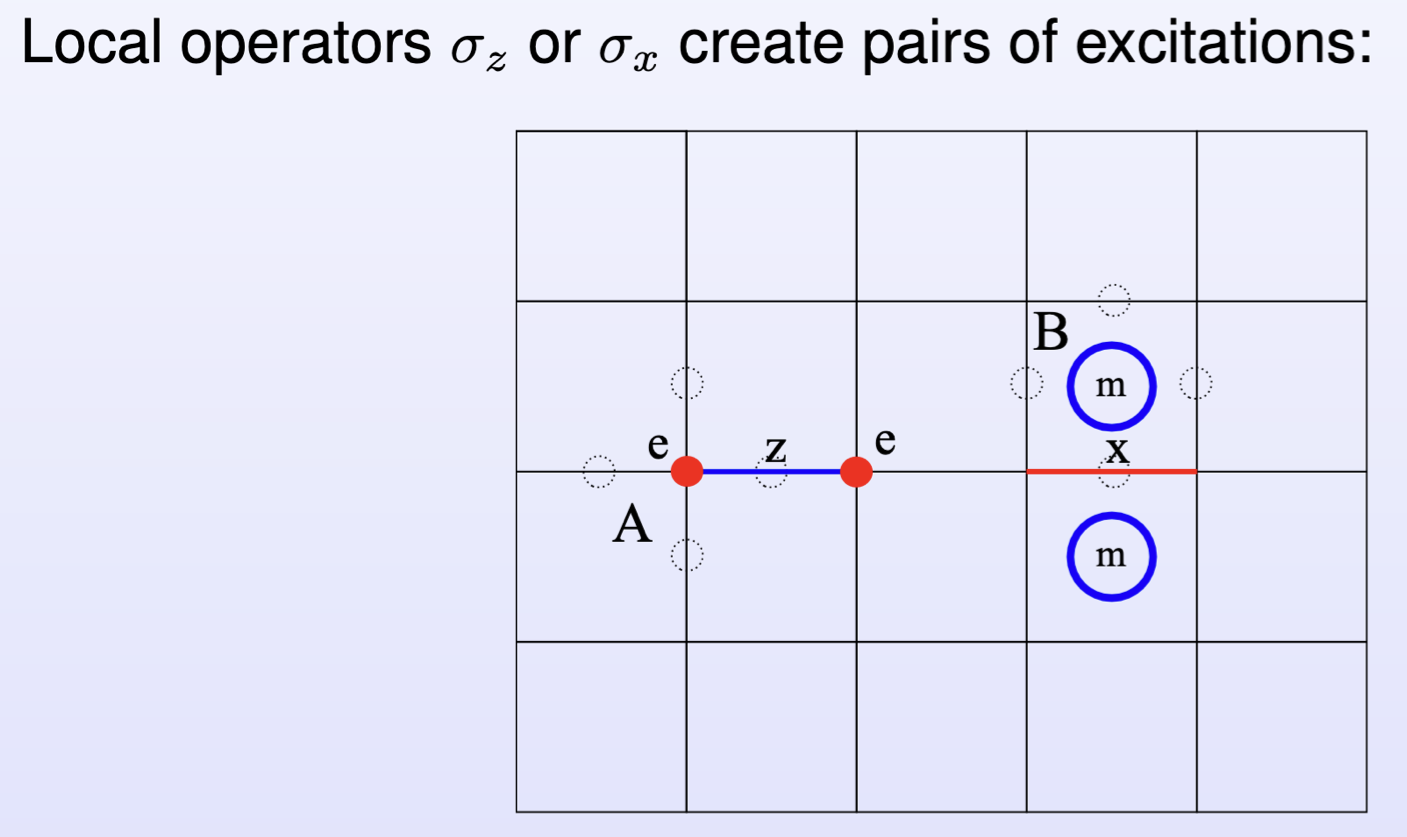
\includegraphics[width=0.6\textwidth]{eandm.png}
     \caption{Pari creation of $e$-excitations and $m$-excitations. Image from \cite{DXN}. }
     \label{fig:label}
 \end{figure}
 The $e$-excitations can be moved by other $Z$s, 
 and the $m$-excitations can be moved by other $X$s. 
 Note that string operators of $X$s are defined on the dual lattice, 
 whereas those of $Z$s are on the original lattice. 
 \begin{figure}[tbp]
 \begin{minipage}[b]{0.48\columnwidth}
 \centering
 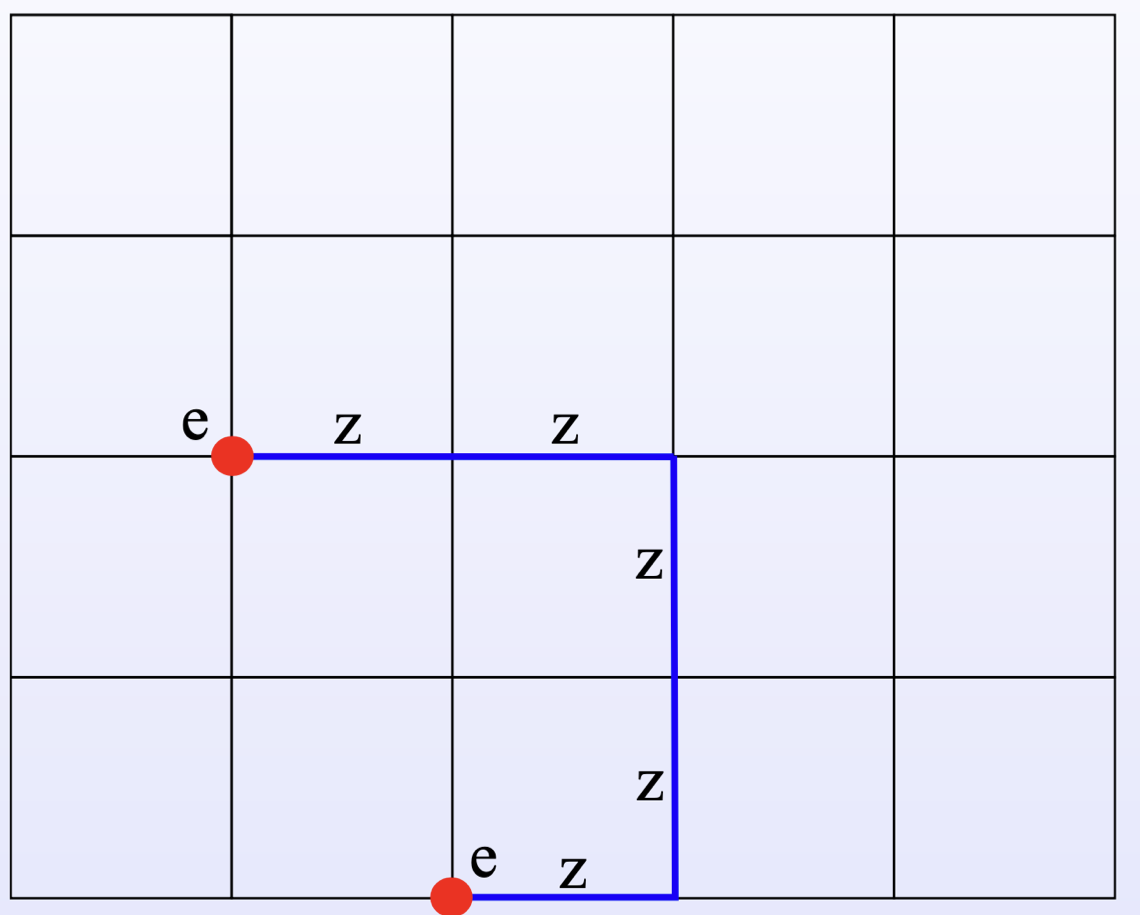
\includegraphics[width=\columnwidth]{e-move.png}
 \caption{$e$-excitations can be moved by $Z$. Image from \cite{DXN}. }
 \end{minipage}
 \hspace{0.04\columnwidth} % ここで隙間作成
 \begin{minipage}[b]{0.48\columnwidth}
 \centering
 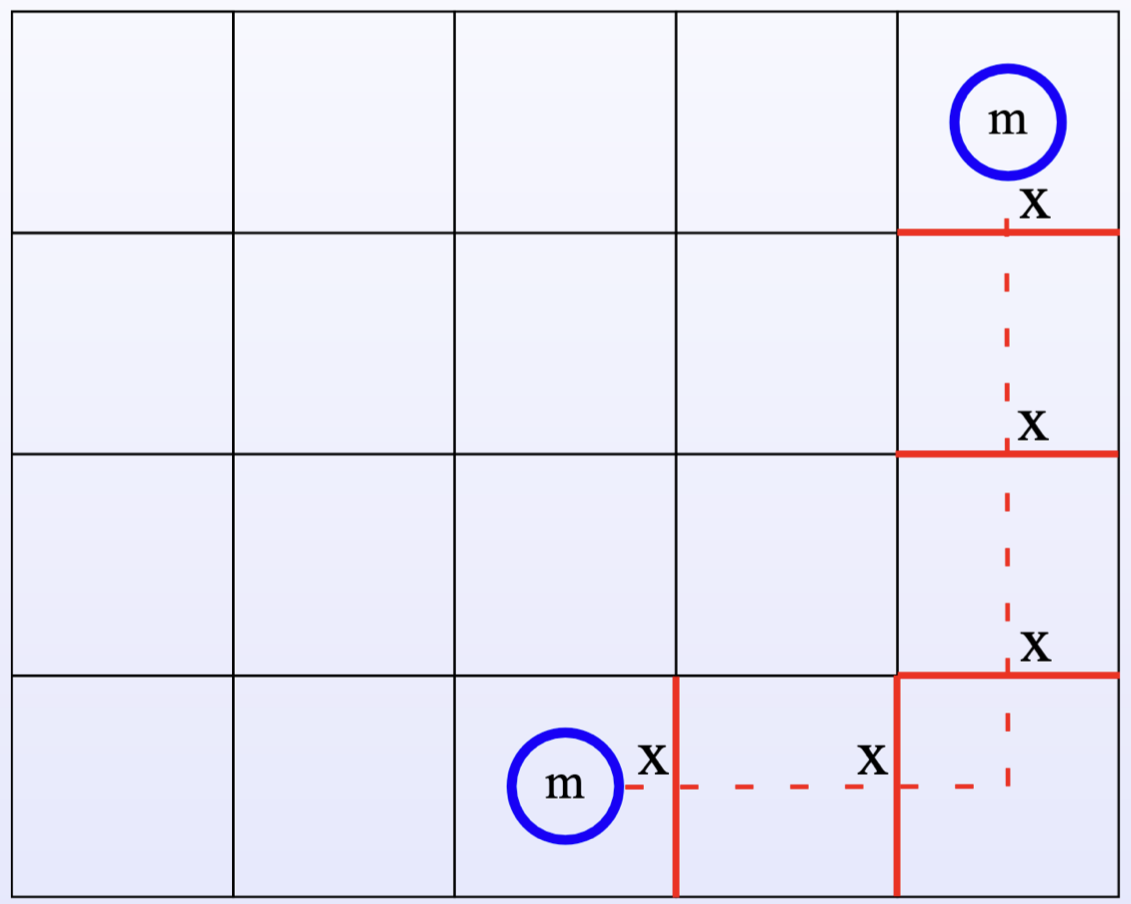
\includegraphics[width=\columnwidth]{m-move.png}
 \caption{$m$-excitations can be moved by $X$. Image from \cite{DXN}. }
 \end{minipage}
 \end{figure}
 We can annihilate the pair of excitations by closing a string of $Z$ or $X$ to form a loop. 
 Therefore, the electric and magnetic charge of such excitations are said to be $\zet_2$-valued. 
 The symmetry of the toric code is generated by closed strings of $\sigma_z$ and $\sigma_x$. 
 There are two types of closed strings: trivial ones and non-trivial ones. 
 Non-trivial ones correspond to the non-trivial homology of the model. 
%ずを載せる%It is known that the ground state of toric code Hamiltonian is degenerated by $4$. 
%This can be considered as the consequence of 
%"$1$-form symmetry breaking of $Z^e_2\times Z^m_2$" 
%(note that the order(位数) of $Z^e_2\times Z^m_2$ is 4). 
%In fact, for example, the charged objects under $Z^e_2$ 
%(i.e. non-contractible closed magnetic loops $W[C]$) 
%have a finite expectation value on the groundstates: 
\subsubsection{anyon braiding}
In toric code model, we have two types of excitations: 
$e$-excitations created by $z$-strings, 
and $m$-excitations by $x$-strings. 
These string excitations can be moved by other $z$s and $x$s freely, 
then they themselves obey a bosonic statistics. \\
 In contrast, when we move the $e$-excitations around $m$-excitations, 
then we will have a non-trivial phase. 
\subsubsection{$1$-form symmetry of toric code}
There are two types of 1-dimensional topological operators defined on the toric code, 
commuting with the Hamiltonian \eqref{TCmodel}. 
They generate $1$-form symmetry $\zet^e_2\times \zet^m_2$.\\
 The symmetry operator of $\zet^e_2$ is the Wilson loop 
$W[C]=\prod_{i\in C}\sigma^z_i$
 (corresponding to \textbf{magnetic string operator} along the non-contractible closed loop), 
and that of $\zet^m_2$ is the 't Hooft loop 
$T[\tilde{C}]=\prod_{i\in \tilde{C}}\sigma^x_i$
(corresponding to \textbf{electric string operator} along the non-contractible closed loop). 
Such kinds of string operators are topological in that 
string operators in the same homology equivalence class 
can be transposed to each other through the multiplication by stabilizers
\footnote{
    The operators $A_j$ (defined on each vertex) and $B_p$ (on each plaquette) are called "stabilizers", 
    since they commute with all the terms in the Hamiltonian \eqref{TCmodel}. 
}. 
\begin{figure}[H]
    \centering
    \resizebox{1\textwidth}{!}{%
    \begin{circuitikz}
    \tikzstyle{every node}=[font=\LARGE]
    \draw [short] (0,15.75) -- (0,10.75);
    \draw [short] (0,10.75) -- (5,10.75);
    \draw [short] (5,15.75) -- (5,10.75);
    \draw [short] (0,15.75) -- (5,15.75);
    \draw [short] (0,14.5) -- (5,14.5);
    \draw [short] (0,13.25) -- (5,13.25);
    \draw [short] (0,12) -- (5,12);
    \draw [short] (1.25,15.75) -- (1.25,10.75);
    \draw [short] (2.5,15.75) -- (2.5,10.75);
    \draw [short] (3.75,15.75) -- (3.75,10.75);
    \draw [ color={rgb,255:red,4; green,51; blue,255}, line width=0.9pt, short] (3.75,15.75) -- (3.75,10.75);
    \node [font=\LARGE, color={rgb,255:red,4; green,51; blue,255}] at (3.75,16.5) {$Z_1$};
    \draw [short] (8.75,15.75) -- (8.75,10.75);
    \draw [short] (8.75,10.75) -- (13.75,10.75);
    \draw [short] (13.75,15.75) -- (13.75,10.75);
    \draw [short] (8.75,15.75) -- (13.75,15.75);
    \draw [short] (8.75,14.5) -- (13.75,14.5);
    \draw [short] (8.75,13.25) -- (13.75,13.25);
    \draw [short] (8.75,12) -- (13.75,12);
    \draw [short] (10,15.75) -- (10,10.75);
    \draw [short] (11.25,15.75) -- (11.25,10.75);
    \draw [short] (12.5,15.75) -- (12.5,10.75);
    \draw [ color={rgb,255:red,4; green,51; blue,255}, line width=0.9pt, short] (12.5,15.75) -- (12.5,10.75);
    \node [font=\LARGE, color={rgb,255:red,4; green,51; blue,255}] at (12.5,16.5) {$Z_1$};
    \draw [short] (17.5,15.75) -- (17.5,10.75);
    \draw [short] (17.5,10.75) -- (22.5,10.75);
    \draw [short] (22.5,15.75) -- (22.5,10.75);
    \draw [short] (17.5,15.75) -- (22.5,15.75);
    \draw [short] (17.5,14.5) -- (22.5,14.5);
    \draw [short] (17.5,13.25) -- (22.5,13.25);
    \draw [short] (17.5,12) -- (22.5,12);
    \draw [short] (18.75,15.75) -- (18.75,10.75);
    \draw [short] (20,15.75) -- (20,10.75);
    \draw [short] (21.25,15.75) -- (21.25,10.75);
    \draw [ color={rgb,255:red,4; green,51; blue,255}, line width=0.9pt, short] (21.25,15.75) -- (21.25,10.75);
    \node [font=\LARGE, color={rgb,255:red,4; green,51; blue,255}] at (21.25,16.5) {$Z'_1$};
    \node [font=\large, color={rgb,255:red,4; green,51; blue,255}] at (3.75,15.25) {$z$};
    \node [font=\large, color={rgb,255:red,4; green,51; blue,255}] at (3.75,14) {$z$};
    \node [font=\large, color={rgb,255:red,4; green,51; blue,255}] at (3.75,12.75) {$z$};
    \node [font=\large, color={rgb,255:red,4; green,51; blue,255}] at (3.75,11.25) {$z$};
    \node [font=\large, color={rgb,255:red,4; green,51; blue,255}] at (12.5,15) {$z$};
    \node [font=\large, color={rgb,255:red,4; green,51; blue,255}] at (12.5,12.75) {$z$};
    \node [font=\large, color={rgb,255:red,4; green,51; blue,255}] at (12.5,11.25) {$z$};
    \node [font=\large, color={rgb,255:red,4; green,51; blue,255}] at (21.25,15) {z};
    \node [font=\large, color={rgb,255:red,4; green,51; blue,255}] at (21.25,12.75) {z};
    \node [font=\large, color={rgb,255:red,4; green,51; blue,255}] at (21.25,11.5) {z};
    \draw [ color={rgb,255:red,4; green,51; blue,255} , fill={rgb,255:red,212; green,227; blue,254}, line width=0.9pt ] (11.25,14.5) rectangle (12.5,13.25);
    \node [font=\large, color={rgb,255:red,4; green,51; blue,255}] at (12.5,14) {$z$};
    \node [font=\large, color={rgb,255:red,4; green,51; blue,255}] at (12,14) {$B_p$};
    \node [font=\large] at (3,14) {$p$};
    \node [font=\large, color={rgb,255:red,4; green,51; blue,255}] at (11.25,14) {$z$};
    \node [font=\large, color={rgb,255:red,4; green,51; blue,255}] at (11.75,14.5) {$z$};
    \node [font=\large, color={rgb,255:red,4; green,51; blue,255}] at (11.75,13.25) {$z$};
    \draw [line width=0.9pt, ->, >=Stealth] (6.25,13.25) -- (7.5,13.25);
    \draw [line width=0.9pt, ->, >=Stealth] (15,13.25) -- (16.25,13.25);
    \draw [ color={rgb,255:red,4; green,51; blue,255}, line width=0.9pt, short] (21.25,14.5) -- (20,14.5);
    \draw [ color={rgb,255:red,4; green,51; blue,255}, line width=0.9pt, short] (20,14.5) -- (20,13.25);
    \draw [ color={rgb,255:red,4; green,51; blue,255}, line width=0.9pt, short] (20,13.25) -- (21.25,13.25);
    \draw [ color={rgb,255:red,255; green,255; blue,255}, line width=0.9pt, short] (21.25,14.5) -- (21.25,13.25);
    \draw [line width=0.5pt, short] (21.25,14.5) -- (21.25,13.25);
    \node [font=\large, color={rgb,255:red,4; green,51; blue,255}] at (20.5,14.5) {z};
    \node [font=\large, color={rgb,255:red,4; green,51; blue,255}] at (20,14) {z};
    \node [font=\large, color={rgb,255:red,4; green,51; blue,255}] at (20.5,13.25) {z};
    \end{circuitikz}
    }%
    \label{fig:my_label}
    \end{figure}
    The corresponding charged operator of $\zet_2^{m}$ is 
    the non-contractable closed electric loop ('t Hooft loop), 
    and that of $\zet_2^e$ is the non-contractable closed magnetic loop (Wlison loop). 
    The action is written as
    \begin{align}
        \label{TCaction}
        W[C] T[\tilde{C}] W[C]^{-1} = e^{i\pi \mathrm{Link}(C, \tilde{C})}T[\tilde{C}], 
    \end{align}
    where $W[C]^{-1}$ is the Wlison loop on the inverse direction of $C$. 
    Intuitively, this action is interpreted as follows: 
    when $W[C]$ and $ T[\tilde{C}]$ are linked, 
    we have to intersect the twoo loops as many as the linking number 
    to "delink" the two. 
    Intersecting the loop of $Z$ and that of $X$ one time gives a phase factor $(-1)$, 
    then we totally get the phase factor above. 
\subsubsection{$1$-form symmetry breaking of GS}
INCOMPLETE\\
\subsubsection{Mixed 't Hooft anomaly of $\zet_2^e\times \zet_2^m$}
\color{red}
INCOMPLETE\\
\color{black}
 As we have seen before, the electric and magnetic $1$-form $U(1)$ symmetries causes
mixed 't Hooft anomaly when they are gauged together. 
The similar thing happens in toric code, but the symmetry here is $1$-form $\zet_2$ instead of $U(1)$. \\
 Consider the action \eqref{TCaction}
\begin{align}
    \label{TCaction}
    W[C] T[\tilde{C}] W[C]^{-1} = e^{i\pi \mathrm{Link}(C, \tilde{C})}T[\tilde{C}].  
\end{align}
If the Linking number is odd, then we have
\begin{align}
    W[C] T[\tilde{C}] = -T[\tilde{C}]W[C]. 
\end{align}
This means that the two symmetry operators do not commute. 
It is problematic when we consider the "gauging" of the two $1$-form symmetry simultaneously. 
%%
%%
\begin{comment}
\newpage
\section{Appendices}
\subsection{A Brief Intro to Toric Code}
\noindent
\tiny
(I think this part should be written by Takumi-san)\\
\normalsize
\subsubsection{topological order}
Generally, a system is said to have topological order if
\cite{DXN}
\begin{itemize}
    \item it has (approximately) degenerate ground states $\{\psi_\alpha\}$ 
    all of which are separated by a finite gap from excited states, 
    \item the degeneracy of $\{\psi_\alpha\}$s are dominated by the topology of the spacetime manifold 
    on which the system is embedded, 
    \item and no loacl operator can either distinguish or induce transitions between two different $\psi_\alpha$s, i.e., 
    \begin{align}
        \langle \psi_1 |\mathcal{O}_{\mathrm{local}} |\psi_2\rangle
    \end{align}
    for any $\mathcal{O}_{\mathrm{local}}$ acting on the Hilbert space. 
\end{itemize}
\subsubsection{toric code Hamiltonian and its groundstates}
The \textbf{toric code} model is constructed on 
an arbitrary dimensioanl lattice (typically square lattice), with periodic boundary condition on both directions 
(i.e. the Hilbert space is on torus $T^2$). 
We put a qubit on every link. 
The Hamiltonian is 
\begin{align}
    H=-\sum_j A_j - \sum_p B_p, 
    \label{TCmodel}
\end{align}
where $j$ and $p$ is the index of site and plaquette respectively, 
$A_{j}\equiv \prod_{l:\mathrm{link~ending~at~j}} Z_l$ is defined for every site $j$, 
and $B_{p}\equiv \prod_{l:\mathrm{bdy~of~p}} X_l$ is for every plaquette $p$. 
$A_j$ and $B_p$ are sometimes called "Gauss law operator" and "flux operator" respectively. \\
 All of those operators $A_j$ and $B_p$ commute with each other since 
they all share an even number (0, 2, or 4) of $X$s and $Z$s 
(so we always have $(-1)^{\mathrm{even}}$ factor). 
Then, we can diagonalize all terms in \label{TCmodel} simultaneously. \\
 Let's consider states whose eigenvalue of $A_j$ is 1 for every $j$. 
For such states, all vertex should be associated with an even number of $X_l$s ending on it. 
The states satisfying this condition are "closed-string states", 
where all lines of electric flux are closed and have no charges to end on. 
Therefore, the groundstate of the toric code model is degenerated as many as the possible closed loop configuration, 
which is the order of the exponential of the system size. \\
Thinking in there are 4 types of loop configurations 
 The groundstates of toric code are said to be in a topological order 
in that no operators can distinguish any of two different operators 
since all of them have the same eigenvalues. \\
\subsubsection{Excited states and anyon braidings}
We are now interested in the excited states of the toric code. 
Remember that the groundstates have eigenvalues $A_v=1$ and $B_p=1$ for all vertices $v$ and plaquettes $p$. 
Then, the excited states are those who violates this condition. \\
 Physically, this corresponds to violating Gauss law or flux conservation. 
In this case, both endpoints of string operators can be regarded as quasiparticles carrying charges. 
The statistics of those quasiparticles are the so-called anyon statistics: 
the time of exchanging two anyons has an essential meaning. \\
 One important property is that those anyons can move freely on a lattice with no energy costs. 
Indeed, as long as the number of quasiparticles does not change, 
the eigenvalues itself remains unchanged. 
Therefore, from the perspective of energy, we cannot distinguish the difference of quasiparticle positions. 
In such a case, the toric code is said to have an error. 
On the contrary, the groundstates of toric code are 
known as the \textit{error-correcting code}. 
\subsection{離散ゲージ理論}
\noindent
\small
This part is originally intended to put in the preliminary of Day1 material, 
so it is written in Japanese. \\
\normalsize
 物理学では, $\mathbb{Z}_2$対称性や$\mathbb{Z}_{N}$対称性のような離散的な対称性が重要な役割を果たすことがある. 
このような離散的な内部対称性を持つ理論, すなわち離散ゲージ理論について簡単に述べる. 
\subsubsection{単体分割可能な時空の場合}
 離散的な変換の場合, 場の各点ごとに異なる変換を施すという事が意味を持たなくなる
(時空座標が連続的で無限個の点からなるのに対して, 変換群の元は離散的で有限個であるため). 
そこで, 場が定義される時空(target space)を単体分割して離散的に取り扱うことで, 
離散群の場合にもゲージ理論を定義できるようにしよう. 
\\
\\
単体分割とは, 微分可能な多様体を, その「基本単位」である単体の和(形式的線型結合)に分割することである. 
$0$次元の単体($0$-単体)は点, $1$次元単体($1$-単体)は線分, $2$次元単体($2$-単体)は三角形, などなど. 
$p$次元の単体は$p$-単体と呼ばれ, これは$(p+1)$個の互いに独立な頂点$(v_0, \cdots, v_p)$を(向きを考慮して)結んで出来る. 
そのため, $p$-単体は独立な頂点の組$(v_0, \cdots, v_p)$によって完全に指定される. 
%イメージほしい, from Nakahara? 
\\
 連続的な場の理論におけるゲージ変換では, 時空上の各点に$G$の元を(あるいは, $\mathfrak{g}$値1-formを)割り当てていた. 
ここではその代わりに, 単体分割された時空において, $p$-単体に対して$G$の元を割り当てる写像(=\textbf{$p$-コチェイン})を考えることにする
(ただし, ここでは$G$はAbel群). 
これは, 連続の場合における$p$-formに対応する. 
このような写像が"コチェイン"と呼ばれる理由は, $p$-コチェインに対して$(p+1)$-コチェインを返す写像
\begin{align}
    \delta c_p (v_0, \cdots, v_{p+1}) = \sum_{i=0}^{p+1}(-1)^i c_p(v_0, \cdots, v_{i-1}, v_{i+1}, \cdots, v_{p+1})
\end{align}
があるためである. 
この$\delta$は, 連続の場合における外微分$d$の対応物であり, $\delta^2=0$を満たす. 
もう少しだけ言うと, 
この$p$-コチェインの$G$係数線型結合($G$-加群)をコチェイン複体(complex)とし, $\delta$をコチェイン写像として, 
$G$係数のコホモロジー群を構成することができる. \\
 微分形式および外微分の「離散的な対応物」を構成できたので, ここに外積代数のような代数構造(つまり, wedge積に相当する演算)を入れることを考えたい. 
いま, Abel群$G$, $H$および$K$に対して, 双準同型$\eta: G\times H\to K$を考える. 
ここで, 双準同型とは, $g\in G$を固定した時に$\eta_g: H\to K$が群準同型になり, 
$h\in H$を固定した時に$\eta_h: G\to K$がやはり準同型になるような二項演算のこと. 
単体分割された時空の頂点の組を$(v_0, \cdots, v_{p+q})$と固定した時, 
$G$値$p$-コチェイン$c_p$と$H$値$q$-コチェイン$d_p$はそれぞれ$G$および$H$の元を返すため, 
双準同型$\eta: G\times H\to K$を用いれば, $K$値の$(p+q)$-コチェインを
\begin{align}
    (c_p \cup_\eta d_q)(v_0, \cdots, v_{p+q}) := \eta(c_p(v_0, \cdots, v_p), d_q(v_{p}, \cdots, v_{p+q}))
\end{align}
として構成できる(右辺における$p$-単体と$q$-単体は, 頂点$v_p$を共有していることに注意). 
このようにして, $p$-コチェインと$q$-コチェインの組に対して$(p+q)$-コチェインを返す対応を
"cup product"$\cup_\eta$と呼び, これは$\eta$の取り方(およびその値域$K$)に明確に依存する. \\
 ゲージ理論では, $G$をゲージ群とした時, 
$H=\hat{G}$, $K=\mathbb{R}/\mathbb{Z}$として(hatはPontryagin双対の意味: 
$\hat{G} = \mathrm{Hom}(G, U(1))$), 
cup productを与える双準同型を
\begin{align}
    \eta(g, \hat{g}) = \alpha\in \mathbb{R}/\mathbb{Z}, ~~
    \alpha = \frac{1}{2\pi i}\log (\hat{g}(g))
\end{align}
によって与える. 
特に, $G=\hat{G}=\zet_n$の場合は, "standard cup product"
\begin{align}
    (c_p \cup d_q)(v_0, \cdots, v_{p+q}) = c_p(v_0, \cdots, v_p)d_q(v_{p}, \cdots, v_{p+q})
\end{align}
を定めることができる. \\
 $D=d+1$次元の離散ゲージ理論の作用は, 一般に
\begin{align}
    2\pi\int a_p \cup_\eta b_{d-p}
    \label{discreteAction}
\end{align}
の形で書け, ゲージ場$a_p$の変換は適当な$G$値$(p-1)$-コチェイン$a_{p-1}$を用いて$a_p \mapsto a_p + \delta a_{p-1}$と書ける
($b_{d-p}$の方も同様). この作用が導く運動方程式(ゲージ場の変換に対する作用の不変性)は, 
\begin{align}
    \delta a_{p} = 0, ~~
    \delta b_{d-p} = 0
\end{align}
となり, これは$a_p$および$b_{d-p}$がコサイクルをなすことを意味する. 
\\
 ところで, 実はこのようなゲージ理論の構成は, 非可換な離散群の場合(例えば, 二面体群$D_6$のようなもの)の場合にはうまくいかない. 
というのも, この構成は時空の単体分割からコチェイン複体を明示的に与えることでなされていたが, 
これが可能なのは$G$がAbel群の時のみである. 
より, 群が非可換な場合は別の工夫が必要になる. 
\subsubsection{もっと一般的な定式化}
上のような単体分割に基づく離散ゲージ理論の構築は実用上(計算上)扱いやすいが, いくつかの問題がある. 
特に, 連続群の場合に考えてきたような"トポロジカル演算子"という描像が, 離散群の場合では微妙になる. 
というのも, 離散群の場合カレント保存則のようなものの存在を保証できないため, 
トポロジカル演算子の定義そのものが微妙になってしまう. \\
 離散群の対称性を持つ場合のゲージ理論の構成を, 
%これ一旦放置していいや
\begin{align}
    Z=\sum_{\pi: P\to X}e^{-S[\pi]}
\label{PFdiscrete}
\end{align}
つまり, 離散ゲージ理論では, あらゆる主$G$束の同型類にわたる和を取って分配関数を与える. 
\end{comment}
\begin{thebibliography}{99}
    \bibitem{SSN} Sakura Sch\"afer-Nameki. 
    ICTP Lectures on (Non-)Invertible Generalized Symmetries. \href{https://arxiv.org/abs/2305.18296}{\texttt{arXiv: 2305.18296}}
    \bibitem{TDBSH} T. Daniel Brennan, Sungwoo Hong. 
    Introduction to Generalized Global Symmetries in QFT and Particle Physics. \href{https://arxiv.org/abs/2306.00912}{\texttt{arXiv: 2306.00912}}
    \bibitem{DXN} Dung Xuan Nguyen.  
    Introduction to Toric code: From higher form symmetry perspective. \href{https://pcs.ibs.re.kr/PCS_Workshops/PCS_Asian_Network_School_&_Workshop_Talks_2023_files/Dung_Xuan_Nguyen.pdf}{slide available here. }
    \bibitem{MG} 
    John McGreevy. TASI Lectures on Symmetries in Quantum Matter. 
    \href{https://mcgreevy.physics.ucsd.edu/talks/2023-TASI-lectures.pdf}{Lecture note available here. }
    \bibitem{SHS} Shu-Heng Shao. 
    \textit{What's Done Cannot Be Undone}: TASI Lectures on Non-Invertible Symmetries
    \href{https://arxiv.org/pdf/2308.00747}{\texttt{arXiv: 2308.00747}}
    \bibitem{SS} Lieb-Schultz-Mattis anomalies as obstructions to
    gauging (non-on-site) symmetries. 
    \href{https://arxiv.org/pdf/2308.05151}{\texttt{arXiv: 2308.05151}}
    \bibitem{LBLBLFTLGDGAPHT} L. Bhardwaj, L. E. Bottini, L. Fraser-Taliente, L. Gladden, D. S. W. Gould, A. Platschorre and H. Tillim. 
    Lectures on Generalized Symmetries. \href{https://arxiv.org/pdf/2307.07547}{\texttt{arXiv: 2307.07547}}
    \bibitem{TD} T. Dumitrescu. Generalized Symmetries and Phases of Gauge Theory 
    (Lecture in IHES, 2024) \href{https://www.youtube.com/watch?v=9pqtqyGtt3M&t=3760s}{YouTube link is accessible here. }
\end{thebibliography}
\end{document}